%% arara directives
% arara: xelatex
% arara: bibtex
% arara: xelatex
% arara: xelatex

%\documentclass{article} % One-column default
\documentclass[twocolumn, switch]{article} % Method A for two-column formatting

\usepackage{preprint}

%% Math packages
\usepackage{amsmath, amsthm, amssymb, amsfonts, algorithm2e, algpseudocode, graphicx, caption, subcaption, multirow}
\RestyleAlgo{ruled}
\graphicspath{ {./Pictures/} }
%% Bibliography options
\usepackage[numbers,square]{natbib}
\bibliographystyle{unsrtnat}
%\usepackage{natbib}
%\bibliographystyle{Geology}

%% General packages
\usepackage[utf8]{inputenc}	% allow utf-8 input
\usepackage[T1]{fontenc}	% use 8-bit T1 fonts
\usepackage{xcolor}		% colors for hyperlinks
\usepackage[colorlinks = true,
            linkcolor = purple,
            urlcolor  = blue,
            citecolor = cyan,
            anchorcolor = black]{hyperref}	% Color links to references, figures, etc.
\usepackage{booktabs} 		% professional-quality tables
\usepackage{nicefrac}		% compact symbols for 1/2, etc.
\usepackage{microtype}		% microtypography
\usepackage{lineno}		% Line numbers
\usepackage{float}			% Allows for figures within multicol
%\usepackage{multicol}		% Multiple columns (Method B)

\usepackage{lipsum}		%  Filler text

 %% Special figure caption options
\usepackage{newfloat}
\DeclareFloatingEnvironment[name={Supplementary Figure}]{suppfigure}
\usepackage{sidecap}
\sidecaptionvpos{figure}{c}

% Section title spacing  options
\usepackage{titlesec}
\titlespacing\section{0pt}{12pt plus 3pt minus 3pt}{1pt plus 1pt minus 1pt}
\titlespacing\subsection{0pt}{10pt plus 3pt minus 3pt}{1pt plus 1pt minus 1pt}
\titlespacing\subsubsection{0pt}{8pt plus 3pt minus 3pt}{1pt plus 1pt minus 1pt}

% ORCiD insertion
\usepackage{tikz,xcolor,hyperref}

\definecolor{lime}{HTML}{A6CE39}
\DeclareRobustCommand{\orcidicon}{
	
\begin{tikzpicture}
	\draw[lime, fill=lime] (0,0) 
	circle [radius=0.16] 
	node[white] {{\fontfamily{qag}\selectfont \tiny ID}};
	\draw[white, fill=white] (-0.0625,0.095) 
	circle [radius=0.007];
	\end{tikzpicture}
	\hspace{-2mm}
}
\foreach \x in {A, ..., Z}{\expandafter\xdef\csname orcid\x\endcsname{\noexpand\href{https://orcid.org/\csname orcidauthor\x\endcsname}
			{\noexpand\orcidicon}}
}
% Define the ORCID iD command for each author separately. Here done for two authors.
\newcommand{\orcidauthorA}{0000-0000-0000-0001}
\newcommand{\orcidauthorB}{0000-0000-0000-0002}
\newcommand{\orcidauthorC}{0000-0000-0000-0003}
\newcommand{\orcidauthorD}{0000-0000-0000-0004}

%%%%%%%%%%%%%%%%   Title   %%%%%%%%%%%%%%%%
\title{Parallel A* project}

% Add watermark with submission status
\usepackage{xwatermark}
% Left watermark
\newwatermark[firstpage,color=gray!60,angle=90,scale=0.32, xpos=-4.05in,ypos=0]{\href{https://doi.org/}{\color{gray}{Publication doi}}}
% Right watermark
\newwatermark[firstpage,color=gray!60,angle=90,scale=0.32, xpos=3.9in,ypos=0]{\href{https://doi.org/}{\color{gray}{Preprint doi}}}
% Bottom watermark
\newwatermark[firstpage,color=gray!90,angle=0,scale=0.28, xpos=0in,ypos=-5in]{*correspondence: \texttt{email@institution.edu}}

%%%%%%%%%%%%%%%  Author list  %%%%%%%%%%%%%%%
\usepackage{authblk}
\renewcommand*{\Authfont}{\bfseries}
\author{Lorenzo Ippolito, Mattia Rosso, Fabio Mirto}


%%%%%%%%%%%%%%    Front matter    %%%%%%%%%%%%%%
\begin{document}

\twocolumn[ % Method A for two-column formatting
  \begin{@twocolumnfalse} % Method A for two-column formatting
  
\maketitle

\begin{abstract}
  ...Here the abstract...
\end{abstract}
%\keywords{First keyword \and Second keyword \and More} % (optional)
\vspace{0.35cm}

  \end{@twocolumnfalse} % Method A for two-column formatting
] % Method A for two-column formatting

%\begin{multicols}{2} % Method B for two-column formatting (doesn't play well with line numbers), comment out if using method A


%%%%%%%%%%%%%%%  Main text   %%%%%%%%%%%%%%%
% \linenumbers

%% %%%%%%%%%%%%%%%%%%%%%%% %%
%% CHAPTER 1: INTRODUCTION %%
%% %%%%%%%%%%%%%%%%%%%%%%% %%
\section{Introduction: about the A* algorithm}
A* is a graph-traversal and path-search algorithm. It is used in many contexts of computer science and 
not only. It can be considered as a general case of the Dijkstra algorithm and it achieves better performaces
with respect to it. It is a Greedy-best-first-search algorithm that uses an heuristic function to guide
itself. What it does is combining:
\begin{itemize}
  \item Dijkstra approach: favore nodes closed to the starting point(source)
  \item Greedy-best-first-search approach: favore nodes closed to the final point(destination)
\end{itemize}
Using the standard terminology we have:
\begin{itemize}
  \item $g(n)$: exact cost of moving from source to n
  \item $h(n)$: heuristic estimated cost of moving from a node n(source included) to the destination
  \item $f(n) = g(n) + h(n)$: in this way we are able to combine the actual cost with the estimated one
\end{itemize}
At each (main loop) iteration the node $n$ that has the minimum $f(n)$ is examinated.
\subsection{Heuristic design}
\paragraph{Premises} We are going to work with weighted oriented graph where $V$ is the set on nodes/vertices
and $E$ is the set of edges of the form $(x,y)$ to indicate that an oriented edge from $x$ to $y$ exists and it
has weight $cost(x, y)$.
\paragraph{Heuristic properties} 
The heurstic function represents the acutal core of the A* algorithm. It represents a prior-knowledge that
we have about the cost of the path from every node (source included) to the destination. 
\begin{itemize}
  \item If we have not this prior information($h(n) = 0 \;\forall n \in V$) we are turning the A* algorithm into
        Dijkstra (this is why A* can be considered as a more general case of Dijkstra algorithm) but we always
        have the guarantee of finding the shortest path. 
  \item Admissible Heuristic: if $h(n) < cost(n, dest) \;\forall n \in V$ (so the we never over-estimate the distance to
        get to the destination from a node $n$) A* will always find the shortest path and the heuristic
        function is called \textit{admissible}. The more inaccurate
        is the estimation the more nodes A* will need to expand (with the upper bound of expanding every
        nodes in the graph if $h(n) = 0$).
  \item Consistent Heuristic: if $h(x) \le cost(x, y) + h(y)$ for every edge $(x, y)$ (so the triangular
        inequality is satisfied) A* has the guarantee to find an optimal path without processing
        any node more than once. 
\end{itemize}
\paragraph{Corner cases} 
\begin{itemize}
  \item Dijkstra: As already discussed if $h(n)=0$ for every node in the graph A* turns into the Dijkstra algorithm.
  \item Ideal: We would obtain a perferct behaviour in case $h(n)$ is exactly equal to the cost of moving from $n$ to
  the destination (A* will only expand the nodes on the best path to get to the destination).
  \item Full greedy-best-first search: if $h(n) \gg g(n)$ than only $h(n)$ plays a role and A* turns into
        a completly greedy-best-first search algorithm.
\end{itemize}

\section{A* project application}
\paragraph{Problem definition} Given a wide range of fields where the A* algorithm can be applied we have choosed the one of
optimal path searching in geographical areas where the goal is to find the minimum distance path from a 
node source to a node destination.

\paragraph{Notation} We work with a weighted oriented graph $G$ that is made of nodes $n \in V$ that represents
road-realated points of interest and edges $(x,y) \in E$ represent the unidirectional connections among these points.
Each edge $(x, y)$ is associated to a weight that is the great-circle distance between $x$ and $y$ measured
in meters.
\paragraph{Benchmark} We will exploit the DIMACS benchmark to make robust estimates of the designed algortithms.
Starting from the FIPS system format files provided we have adopted them (as better explained in section ...) to provide
to the algorithms a file containing information structured as:
\begin{itemize}
  \item Nodes: each node $n$ is defined as $(index, longitude, latitude)$ where $index$ is a natural progressive
        number starting from $0$ used to univocally identify the node and $(longitude, latitude)$ are the geographical
        coordinates of the node.
  \item Edges: each edge $(x, y)$ is defined as $(x, y, weight)$ that represent a unidirectional connection
        from $x$ to $y$ (a road) with length $weight$ (great-circle distance from $x$ to $y$).
\end{itemize}
\subsection{Heuristic function: the great-circle distance}
As previoulsly discussed the A* needs an admssible and consistent heuristic to properly work and this
function is tipically problem-specific. Given the type of problem we are going to apply A* to we are going
to use a measure of geographical distance that extends the concept of heuclidean distance between two points:
the great circle distance (that is the shortest distance over the earth surface measured along the
earth surface itself).
\begin{figure}[ht!]
  \centering
  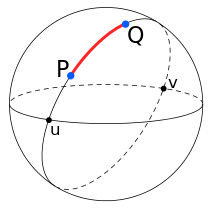
\includegraphics[width=0.5\linewidth]{haversine.png}
  \caption{Great circle distance from P to Q}
  \label{haversine}
\end{figure}
We will employee the Haversine formula to compute the distance from node $(\phi_1,\lambda_1)$
and $(\phi_1,\lambda_1)$ where $\phi$ is the latitude and $\lambda$ is the longitude:
\begin{center}
  $d = R \cdot c$\\
  where $c = 2 \cdot atan2(\sqrt{a},\sqrt{1-a})$\\
  $a = sin^2\Big({\frac{\Delta \phi}{2}}\Big) + cos(\phi_1) \cdot cos(\phi_2) \cdot sin^2\Big({\frac{\Delta \lambda}{2}}\Big)$
  \\$R$ is the earth radius that we have fixed to $R=6.371km$
\end{center}

\section{Graph file input}
\paragraph{File input format} 
Now we start discussing the A* alogorithm implementation and to do that we need to specify which 
types of files we will need to provide to the algorithm to load the graph of interest. Each file has 
the format:
\begin{itemize}
    \item First line: the number of nodes $N[int]$
    \item N following lines: nodes appearing as $(index[int], longitude[double], latidue[double])$
    \item E following lines (with E unknown): edges appearing as $(x[int], y[int], weight[double])$
\end{itemize}
\paragraph{Random test graph} We have tested the designed algorithms also a random generated graph that
is build starting from: 
\begin{itemize}
  \item Which path we want to find: given the couple (source, destination) it is generated a graph of
        $max(source, destination) + 1$ nodes.
  \item How many paths at most have to be generated from source to destination
  \item The maximum length of these paths (that will be randomly chosen for each path)
\end{itemize}
In this way we have ad-hoc files to stress the algorithm having the guarantee that more than one path
exists from source to destination (other more standart approach exist for random graph generation but we
have implemented this custom one for this reason). To be consistent with benchmark files also these
random graphs represents geographic points with longitude and latitude.
\paragraph{DIMACS benchmark} 
The benchmark files we have used come from the DIMACS benchmark. Here each geographic map is described by:
\begin{itemize}
  \item \textit{.co} file: a file containing the coordinates of the nodes following the FIPS system notation
  \item \textit{.gr} file: a file containing the edges and the relative weight(distance) expressed in meters
\end{itemize}
The generation of a file consistent with the format described above happens by merging these files 
into a new one (in binary format). One of the challenge we are going to undertake is the one of
parallelizing the reading of these huge files (that we will show having an high impact in terms of
execution time over the overall A* algorithm).
\paragraph{Test paths}
To analyze the performance of the different versions of A* algorithms we have used these paths:
\begin{table}[ht!]
	\caption{Test paths for A*}
	\centering
	\begin{tabular}{ |l|l|l|l| }
		\hline
		Nodes & Edges & Source & Dest \\ 
    \hline
		\multicolumn{4}{ |c| }{\bf{Random map}} \\
		\hline
		\multirow{1}{*}{}
		 101& - & 0 & 100\\
		\hline
		\multicolumn{4}{ |c| }{\bf{California(BAY) map}} \\
		\hline
		\multirow{1}{*}{}
		321270& 800172 & 321269 & 263446\\
		\hline
		\multicolumn{4}{ |c| }{\bf{Florida(FLA) map}} \\
		\hline
		\multirow{1}{*}{}
		1070376& 2712798 & 0 & 103585\\
		\hline
	\end{tabular}
\end{table}
The paths on benchmark graphs BAY and FLA have been choosen ad-hoc to traverse the entire map with
a reasonable long path.
\begin{figure}[ht!]
  \centering
  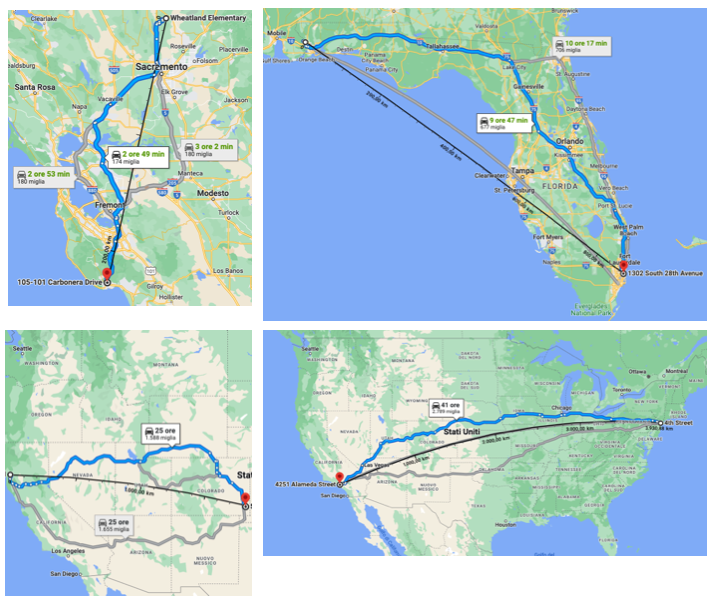
\includegraphics[width=0.75\linewidth]{google_maps.png}
  \caption{Test paths on BAY(left) and FLA(right)}
  \label{testpaths}
\end{figure}

\section{Sequential A* Algorithm}
(Explanation)

\subsection{Psedocode}
\SetKwComment{Comment}{/* }{ */}
\begin{algorithm} 
\caption{An algorithm with caption}\label{alg:two}
\KwData{$n \geq 0$}
\KwResult{$y = x^n$}
$y \gets 1$\;
$X \gets x$\;
$N \gets n$\;
\While{$N \neq 0$}{
  \eIf{$N$ is even}{
    $X \gets X \times X$\;
    $N \gets \frac{N}{2}$ \Comment*[r]{This is a comment}
  }{\If{$N$ is odd}{
      $y \gets y \times X$\;
      $N \gets N - 1$\;
    }
  }
}
\end{algorithm}

\subsection{C Implementation}
(Explain the details of the input file and of the main data structures used)

\subsection{Results}
(Results of sequential reading + A* sequential on random, BAY, FLA)
(Table with numbers)

\section{A* and Dijkstra: a comparison}
(Explanation)

\subsection{Results}
(Picture A* vs Dijkstra on BAY and FLA)

\section{Parallel reading of the input file}
(Motivation of parallel reading)
\subsection{Parallel Read: approach 1}
(Explanation)
\subsection{Parallel Read: approach 2}
(Explanation)
\subsection{Parallel Read: approach 3}
(Explanation)
\subsection{Results}
(Plots of parallel reading vs sequential reading)

\section{Parallel A*: two examinated approaches}
(Explanation)
\subsection{First Attempt In Parallelizing A*}
(Explanation + Pseudocode?)
\subsection{HDA*}
(Introduction + map with colored points)
\subsubsection{Message Passing Model}
(Explanation + Pseudocode?)
\subsubsection{Shared Address Space Model}
\paragraph{Barrier(SAS-B)}
(Explanation + Pseudocode?)
\paragraph{Barrier(SAS-SF)}
(Explanation + Pseudocode?)
\subsection{Results}
(Plots with the comparison of all the models with sequential A* on
random, BAY, FLA)

\section{Complete Results}
(Tables with numbers)

\section{Final Considerations}
(Comments)

\section{DIMACS Benchmark}
(More detailed explanation of the input format of the benchmarks)

\section{Future Works}
(Possible improvements)




%%%%%%%%%%%% Supplementary Methods %%%%%%%%%%%%
%\footnotesize
%\section*{Methods}

%%%%%%%%%%%%% Acknowledgements %%%%%%%%%%%%%
%\footnotesize
%\section*{Acknowledgements}

%%%%%%%%%%%%%%   Bibliography   %%%%%%%%%%%%%%
\normalsize
\bibliography{references}

%%%%%%%%%%%%  Supplementary Figures  %%%%%%%%%%%%
%\clearpage

%%%%%%%%%%%%%%%%   End   %%%%%%%%%%%%%%%%
%\end{multicols}  % Method B for two-column formatting (doesn't play well with line numbers), comment out if using method A
\end{document}